\documentclass{article}%
\usepackage[T1]{fontenc}%
\usepackage[utf8]{inputenc}%
\usepackage{lmodern}%
\usepackage{textcomp}%
\usepackage{lastpage}%
\usepackage{authblk}%
\usepackage{graphicx}%
%
\title{Promoter methylation of RASSF1A modulates the effect of the microtubule{-}targeting agent docetaxel in breast cancer}%
\author{Beth Barnes}%
\affil{Department of Traditional Chinese Medicine, Peking Union Medical College Hospital (PUMCH), Peking Union Medical College (PUMC), Chinese Academy of Medical Sciences, Beijing 100730, China}%
\date{01{-}01{-}2012}%
%
\begin{document}%
\normalsize%
\maketitle%
\section{Abstract}%
\label{sec:Abstract}%
Best available science predicts that the right molecules will enable a breast cancer therapy to be more effective and be at arms length from breast cancer cells, according to researchers at the Dana{-}Farber Cancer Institute and Dana{-}Farber Cancer Institute, both in Boston.\newline%
IMAGE: Dana{-}Farber\newline%
For the purpose of this research, the Dana{-}Farber researchers focused on drug interaction properties that are connected to MAK{-}based kinase inhibitors and their ability to interact with estrogen{-}receptor (ER) or pre{-}cancerous cells and inhibit tumor growth. These studies discovered ways to reduce the drug interaction activity in a mutation of the MMK1 (RNA{-}Associated Molecule) gene using the Novel NSCLC Target Strategy program to determine how MK is using the LKB1{-}dependent kinase pathway to initiate tumor growth. MK has been programmed into cancer cells by single RNA molecules, just like an aspirin. MK originates in the region of the RNA molecule TIM{-}14, which is non{-}toxic and non{-}drug active. MK inhibits cancer growth by inhibiting the activity of cancer{-}resistant tumor cell genes called phosphorylation receptors in advanced tumors.\newline%
While these laboratory findings are preliminary, the findings give hope that drugs and other molecular inhibitors that interfere with MK by inducing the LKB1{-}dependent kinase pathway and regulating its interactions with the ER receptors may be useful in stimulating a PI3K pathway to kill LK targets or tumor{-}specific Gluco{-}Anchoryl{-}2 (GAL) expressed blood vessels and to prevent tumors from metastasizing.\newline%
Dr. Stewart Lotz, of Dana{-}Farber, principal investigator on the study and Professor of Pathology and Molecular Genetics at the Dana{-}Farber Cancer Institute, said, These results are especially exciting because they provide evidence that certain receptor overexpression (receptor activation) components of the MK kinase group may be one step down on the pathway of MAK, allowing binding of these genes to some of the most toxic cancer stem cells in the body.\newline%
The research team found that inhibiting the receptor LKB1 (RNA{-}Associated Molecule) of the MAK pathway stimulated activation of MMK (RNA{-}Associated Molecule) ofMAK6, an important MMK in vivo/environmental membrane protein. IMPA6 has a similar effect on MMK6 in cancer patients. The researchers conclude that MAK makes a world of difference for MMK inhibitors in a pathway that has a great deal of activity targeting advanced cancers.

%
\subsection{Image Analysis}%
\label{subsec:ImageAnalysis}%


\begin{figure}[h!]%
\centering%
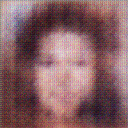
\includegraphics[width=150px]{500_fake_images/samples_5_214.png}%
\caption{A Man With A Beard And A Beard Wearing A Tie}%
\end{figure}

%
\end{document}